\documentclass[11pt,twoside,b5paper]{book}

\usepackage[b5paper,tmargin=1cm,bmargin=1.5cm, innermargin=2cm]{geometry}

\usepackage{fancyhdr}
\pagestyle{plain}
\fancyhf{}


\fancypagestyle{mainmatter}{
\rhead{Why R? 2017}
\lhead{Książka konferencyjna}
\rfoot{\thepage}
}

\usepackage{emptypage}
\usepackage{enumitem}

\usepackage{subfiles}
\usepackage{hyperref}
\usepackage{titlesec}

\usepackage{longtable} 
\usepackage{pdflscape} 
\usepackage{afterpage}
\usepackage{parskip}
\usepackage{wrapfig}
\usepackage{graphicx}
\usepackage{caption}
\usepackage{subcaption}

\usepackage{imakeidx}
\makeindex[name=a,title=Indeks nazwisk,intoc=true]

\usepackage[utf8]{inputenc}
\usepackage[T1]{fontenc}
\usepackage{eurosym}
\usepackage{amsfonts, amsmath, hanging, hyperref, parskip, times}
\usepackage[numbers]{natbib}

\hypersetup{
	colorlinks,
	linkcolor=black,
	urlcolor=black,
	citecolor=black
}

\usepackage{pdfpages}

%\let\section=\subsubsection
\newcommand{\pkg}[1]{{\normalfont\fontseries{b}\selectfont #1}}
\let\proglang=\textit
\let\code=\texttt
\newcommand{\atitle}[1]{\begin{center}{\bf \LARGE #1}\end{center}}
\newcommand{\affiliations}{\footnotesize\centering}
\newcommand{\keywords}{\paragraph{Keywords:}}
\newcommand{\opiswarsztatu}{\subsubsection{Opis warsztatu}\noindent \small}
\newcommand{\planwarsztatu}{\subsubsection{Plan warsztatu}\small}
\newcommand{\pakiety}{\subsubsection{Wymagane pakiety}\noindent \small}
\newcommand{\umiejetnosci}{\subsubsection{Wymagane od uczestników umiejętności i wiedza}\noindent \small}
\newcommand{\wymagania}{\subsubsection{Wymagania wstępne do wykonania przed warsztatem}\noindent \small}
\newcommand{\sylwetkaprowadzacego}{\subsubsection{Sylwetka prowadzącego}\noindent \small}
\newcommand{\packages}{\subsubsection{R packages:}}
\newcommand{\bio}{\subsubsection{Bio} \small}


\renewcommand*\contentsname{Spis treści}

\newcommand{\mychapter}[1]{\chapter{#1} \title{#1} \newpage}

\usepackage{titlesec}
\titleformat{\chapter}[display]   
{\normalfont\Huge\bfseries}{\chaptertitlename\ \thechapter}{80pt}{\LARGE}   
\titlespacing*{\chapter}{0pt}{0pt}{0pt}

\providecommand{\tightlist}{%
	\setlength{\itemsep}{0pt}\setlength{\parskip}{0pt}}

% \setlength{\topmargin}{-25mm}
\setlength{\oddsidemargin}{-2mm}
% \setlength{\textwidth}{165mm}
% \setlength{\textheight}{250mm}

\titleformat{\chapter}[display]
{\normalfont\bfseries}{}{0pt}{\huge}

\titleformat{\section}[block]
{\LARGE\bfseries}{}{0pt}{\titlerule\\}[\vspace{2pt}\titlerule]

\titlespacing\subsubsection{0pt}{12pt plus 4pt minus 2pt}{0pt plus 2pt minus 2pt}
%\titleformat{\section}[block]
%{\Large\bfseries\filcenter}{}{1em}{}

\setcounter{secnumdepth}{0}
\setcounter{tocdepth}{1}

\title{Why R? 2017}
\author{Ogólnopolska Konferencja Użytkowników R}
\date{Warszawa, 27-29 września 2017}

\begin{document}

\includepdf{figs/okladkaprzodniebieska.pdf}
% \cleardoublepage

\clearpage

\frontmatter
\maketitle

\begin{small}
\cleardoublepage
\pagenumbering{gobble}
\tableofcontents
\cleardoublepage
\pagenumbering{arabic} 
\end{small}

\mainmatter

\chapter*{Komitet organizacyjny}
\par
\subfile{misc/organizatorzy.tex}

\chapter*{Organizatorzy}
\subfile{abstracts/O01_MiNI.tex}
%\subfile{abstracts/O02_PW.tex}
\newpage
\subfile{abstracts/O03_MI2.tex}
\subfile{abstracts/O04_KNDS.tex}

\chapter*{Partnerzy społecznościowi}
\subfile{abstracts/PS01_Sztychta.tex}
\subfile{abstracts/PS02_Tableau.tex}
\subfile{abstracts/PS19_QuantFin.tex}
\newpage
\subfile{abstracts/PS03_STWUR.tex}
\subfile{abstracts/PS04_eRka.tex}
\newpage
\subfile{abstracts/PS05_trigeR.tex}
\subfile{abstracts/PS06_RLadies.tex}
\subfile{abstracts/PS07_SER.tex}
\subfile{abstracts/PS08_PAZUR.tex}
\subfile{abstracts/PS09_FuRBS.tex}
\subfile{abstracts/PS10_Stacja.tex}
\subfile{abstracts/PS11_Lach.tex}
\subfile{abstracts/PS12_DataScience.tex}
\subfile{abstracts/PS13_SmarterPoland.tex}
\subfile{abstracts/PS14_DataScienceWarsaw.tex}
\subfile{abstracts/PS15_Microsoft.tex}
\subfile{abstracts/PS16_SQL.tex}
\subfile{abstracts/PS17_datahero.tex}
\subfile{abstracts/PS18_DSLodz.tex}


\chapter*{Wstęp}
  \textit{Nie ukrywam ogromnych nadziei jakie wiążę z tym wydarzeniem. Jest to wyjątkowa szansa na wzmocnienie całej polskiej społeczności analityków danych i pasjonatów języka R. Takie spotkania są potrzebne nam wszystkim, na co dzień zmagającym się z~wyzwaniami stawianymi przez świat analizy danych.}

  \textit{To tu praktycy ze środowiska biznesowego mogą pochwalić się osiągnięciami i zasięgnąć rady od kolegów z branży. To tu naukowcy i przedstawiciele świata akademickiego mają możliwość przedstawienia wyników badań oraz projektów, nad którymi pracują.\\ Ostatecznie, to tu wszyscy rozumiemy, że tylko poprzez wspólną wymianę doświadczeń i~przemyśleń jesteśmy w stanie razem utrzymywać renomę polskich specjalistów w dzienie analizy danych na światowym poziomie.}

\begin{flushright}
\ \\ \ \\ \ \\ \ \\
Marcin Kosiński \\
Przewodniczący Komitetu Organizacyjnego \\
Ogólnopolskiej Konferencji Użytkowników R  \\
Why R? 2017 \\
\ \\
Współorganizator \\
Warszawskich Spotkań Entuzjastów R \\
\ \\
Pasjonat R, analizy danych \\
i organizacji wydarzeń

\end{flushright}

\chapter*{Plan konferencji}
\noindent\makebox[\textwidth]{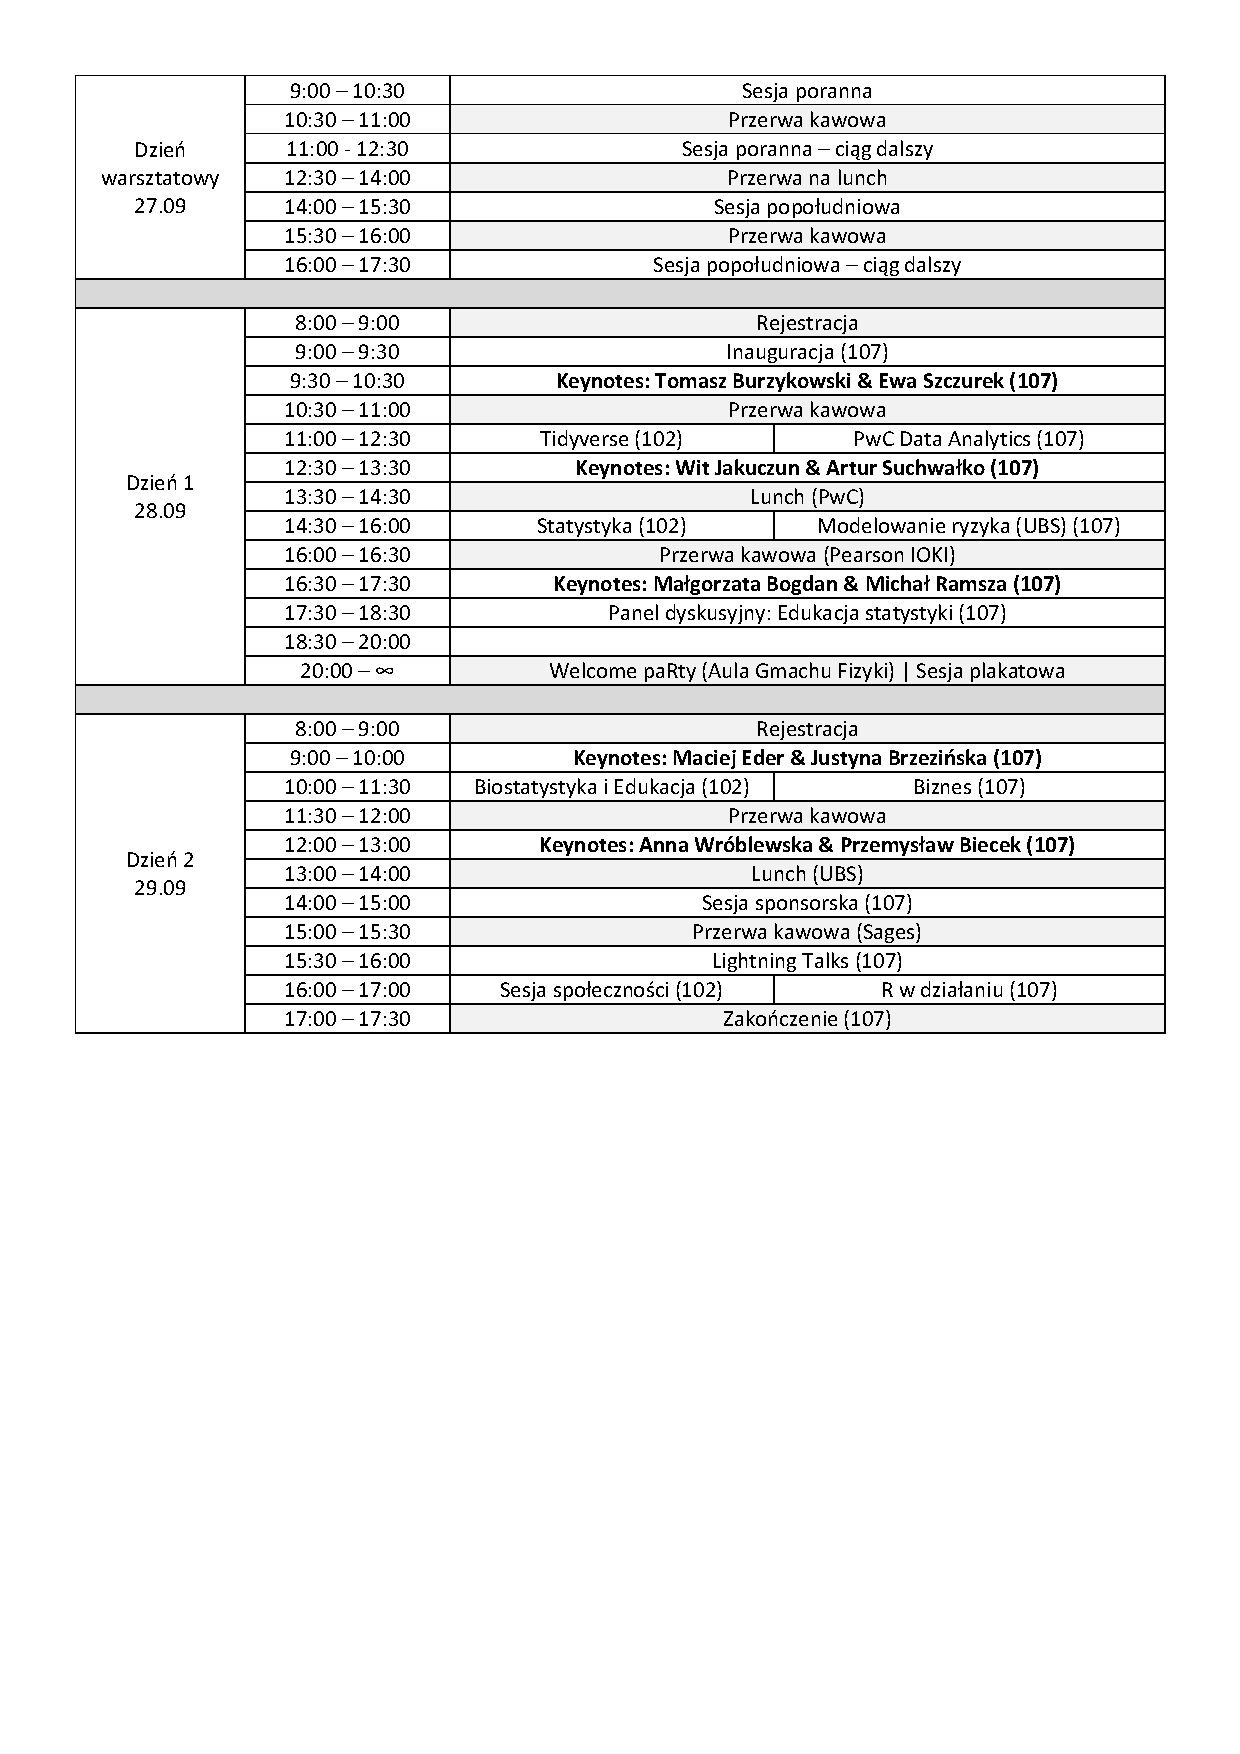
\includegraphics[width=1.25\textwidth,trim=0cm 10cm 0cm 0cm,clip]{figs/plan.pdf}}

\chapter*{Plan warsztatów}
\noindent\makebox[\textwidth]{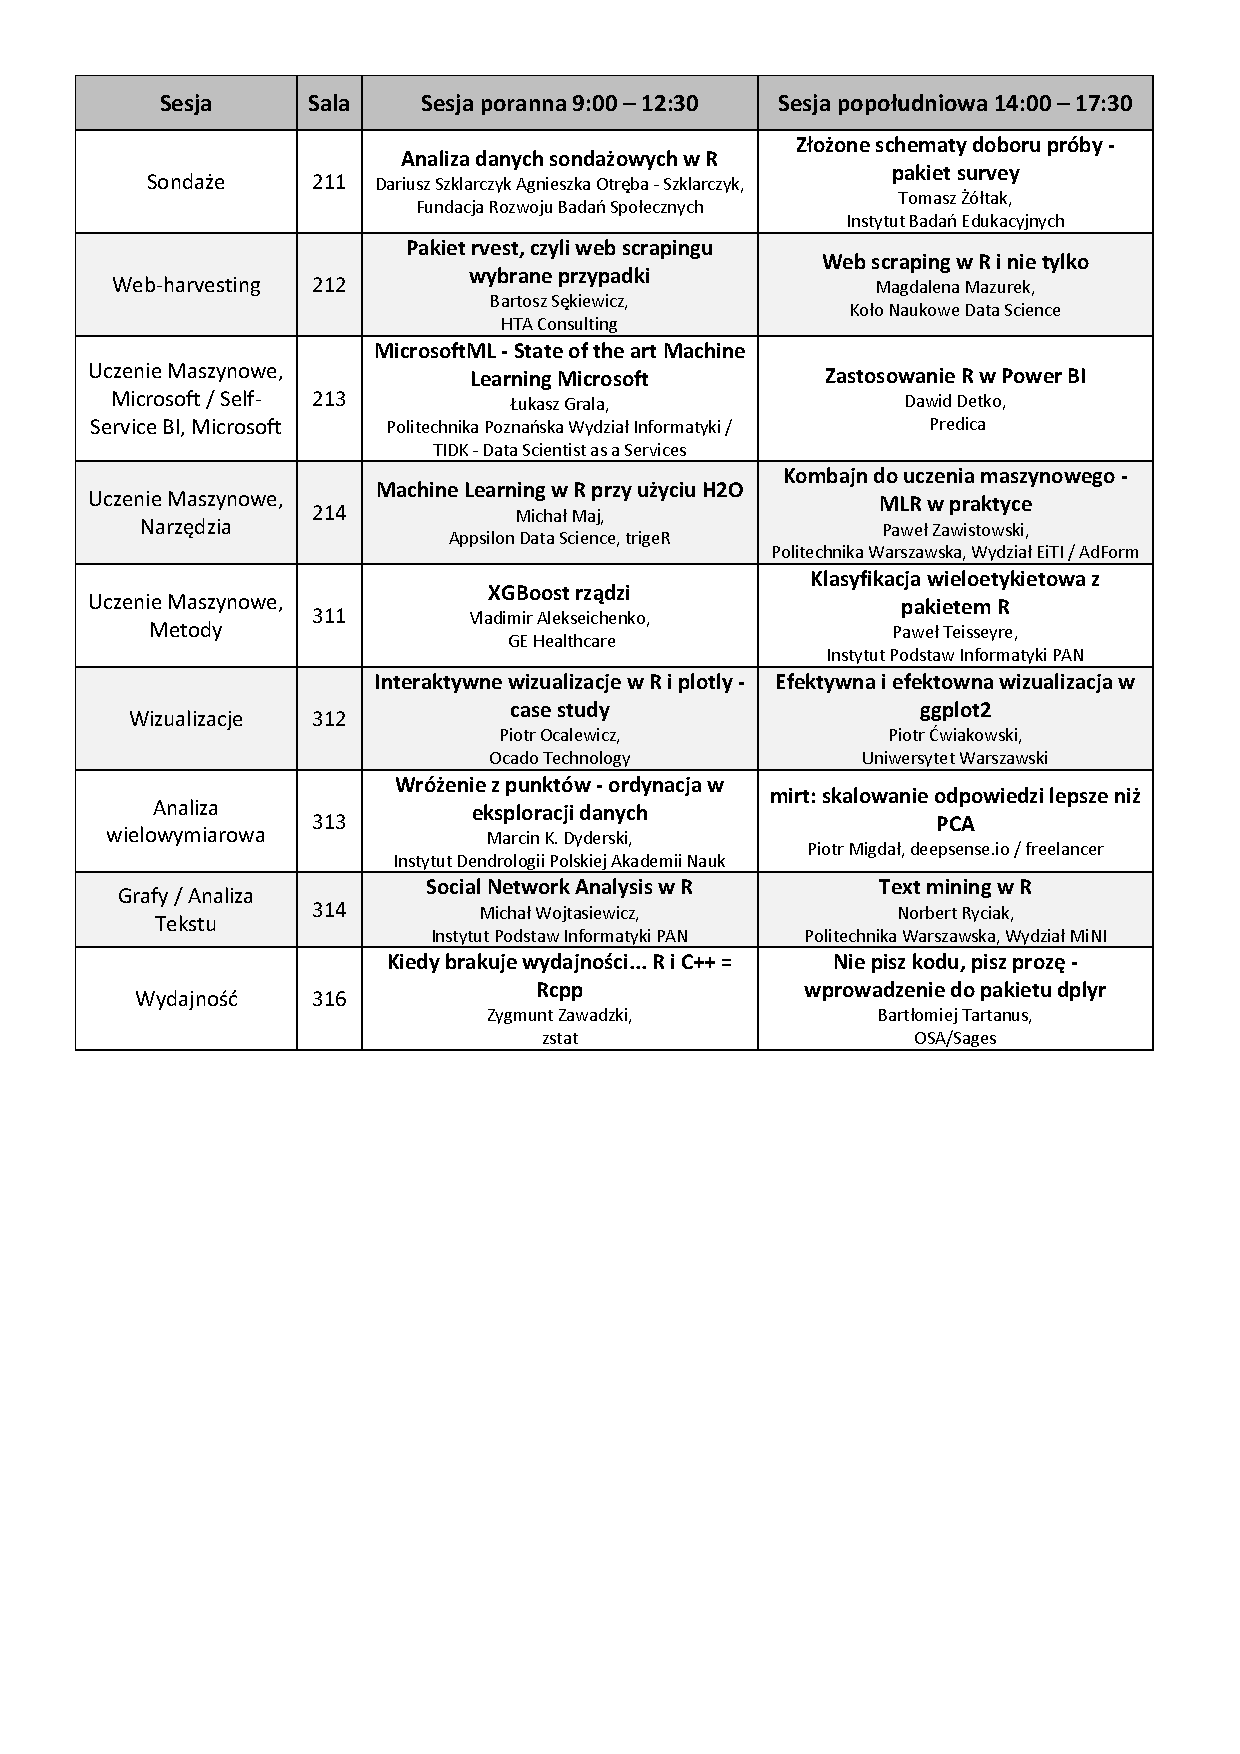
\includegraphics[width=1.25\textwidth,trim=0cm 10cm 0cm 0cm,clip]{figs/plan_warsztaty.pdf}}

\chapter{Wykłady plenarne}{}
\newpage  
\subfile{abstracts/04_Burzykowski.tex}
\newpage
\subfile{abstracts/09_Szczurek.tex}
\newpage
\subfile{abstracts/06_Jakuczun.tex}
\newpage
\subfile{abstracts/08_Suchwalko.tex}
\newpage
\subfile{abstracts/02_Bogdan.tex}
\newpage
\subfile{abstracts/07_Ramsza.tex}
\newpage
\subfile{abstracts/05_Eder.tex}
\newpage
\subfile{abstracts/03_Brzezinska.tex}
\newpage
\subfile{abstracts/10_Wroblewska.tex}
\newpage
\subfile{abstracts/01_Biecek.tex}






\chapter{Sesje}{\LARGE}
\newpage
\section{PwC Data Analytics}
\begin{minipage}[t]{0.915\textwidth}
	\center     
    
\includegraphics[width=100px]{img/PwC_logo_new.png} 
\end{minipage}

PwC to czwarta najsilniejsza marka świata według badania Brand Finance, a jednocześnie zwycięzca w 3 rankingach Warsaw Busiuness Journal: doradztwa biznesowego, podatkowego oraz usług audytowo- księgowych.

Firma PwC kieruje się w swojej działalności trzema głównymi wartościami: jakością i doskonałością, pracą zespołową oraz przywództwem. Świadczy usługi z zakresu audytu, doradztwa biznesowego, podatkowego i prawnego, jak również w obszarze digital transformation. Jest obecna w 157 krajach zatrudniając ponad 233 tysięcy pracowników na całym świecie.

W Polsce PwC zatrudnia zespół blisko 3 500 pracowników w ośmiu miastach: w Gdańsku, Katowicach, Krakowie, Łodzi, Poznaniu, Rzeszowie, Wrocławiu i Warszawie.
\subfile{abstracts/PC01.tex}
\subfile{abstracts/PC02.tex}\newpage
\subfile{abstracts/PC03.tex}
\newpage
\section{Tidyverse}{}
\subfile{abstracts/T01_Mierzwa.tex}
\subfile{abstracts/R05_Kochanski.tex}
\subfile{abstracts/T03_Mlodozeniec.tex}
\subfile{abstracts/T04_Potocka.tex}
\subfile{abstracts/T05_Sobczyk.tex}
\section{Modelowanie Ryzyka (UBS)}
\begin{minipage}[t]{0.915\textwidth}
	\center     
    
\includegraphics[width=100px]{img/ubs.png} 
\end{minipage}

UBS jest jedną z największych instytucji finansowych na świecie, z ponad 150-letnią historią. Działalność firmy koncentruje się na trzech głównych obszarach: zarządzaniu majątkiem, zarządzaniu aktywami oraz bankowości inwestycyjnej. Zatrudniamy ponad 60000 osób w ponad 50-ciu krajach. Główna siedziba UBS znajduje się w Szwajcarii, natomiast w biurach w Krakowie i we Wrocławiu pracownicy współpracują w ramach zespołów zlokalizowanych w różnych regionach Europy i świata.

UBS tworzy środowisko ludzi zafascynowanych modelowaniem, którzy chętnie dzielą się swoją wiedzą, a język R jest szeroko używany wewnątrz UBS w obszarze modelowania ryzyka.
\subfile{abstracts/MR01_Ochotny.tex}
\subfile{abstracts/MR02_Wrobel.tex}
\subfile{abstracts/MR03_Kowalczyk.tex}
\newpage
\section{Statystyka}
\subfile{abstracts/MS01_Wojcik.tex}
\subfile{abstracts/MS02_Dyderski.tex}
\subfile{abstracts/R04_Bigos.tex}
\subfile{abstracts/MS04_Slomczynski.tex}
\subfile{abstracts/MS05_Grala.tex}
\newpage
\section{Biostatystyka i Edukacja}
\subfile{abstracts/BIO01_Stankiewicz.tex}
\subfile{abstracts/BIO02_Gosiewska.tex}
\subfile{abstracts/BIO04_Kosinski.tex}
\subfile{abstracts/BIO05_Oles.tex}
\subfile{abstracts/R02_Melcer.tex}
\newpage
\section{Biznes}
\subfile{abstracts/BIZ01_Olszewski.tex}
\subfile{abstracts/BIZ02_Skrzydlo.tex}\newpage
\subfile{abstracts/BIZ03_Zoltak.tex}
\subfile{abstracts/BIZ04_Jedrzejewski.tex}
\subfile{abstracts/BIZ05_Martsenyuk.tex}
\newpage
\section{Społeczności}
\textbf{Dla kogo ?} \\
Dla wszystkich zaangażowanych w tworzenie społeczności R w Polsce. Zarówno dla osób, które takie grupy prowadzą, jak również dla tych którzy chcą utworzyć społeczność entuzjastów R w swojej okolicy :)

\textbf{Dlaczego ?}\\
Grupy pasjonatów odgrywają ogromną rolę w popularyzacji R. Celem każdego ze spotkań jest wymiana wiedzy i doświadczeń pomiędzy obecnymi i nowymi użytkownikami, kształcenie oraz networking. W Polsce aktywnie działa 6 grup. W trakcie sesji chcielibyśmy pomóc w znalezieniu inspiracji do dalszego działania oraz ułatwić wymianę doświadczeń związanych z organizacją społeczności skupiających entuzjastów R w Polsce.

\textbf{Czego można się spodziewać ?}\\
Żywiołowej dyskusji pomiędzy przedstawicielami istniejących społeczności R w Polsce, pod kontrolą charyzmatycznego prowadzącego :)
\newpage
\newpage
\chapter{Lightning Talks}{\LARGE \textit{Sala 107 - Chairman: Marcin Kosiński}}
\subfile{abstracts/R01_Otmianowski.tex}
\subfile{abstracts/L01_Chmura.tex}
\subfile{abstracts/L02_Czernecki.tex}
\subfile{abstracts/L03_Bielski.tex}
\subfile{abstracts/L05_Lodzikowski.tex}
\subfile{abstracts/L06_Staniak.tex}
\newpage
\chapter{Sesja plakatowa}{\LARGE \textit{Aula Gmachu Fizyki PW}}
\subfile{abstracts/P01_Pawlik.tex}
\subfile{abstracts/P02_Czortek.tex}
\subfile{abstracts/P03_Pawlowska.tex}
\newpage
\chapter{Warsztaty}{}
\subfile{abstracts/W01_Szklarczyk.tex}
\newpage
\subfile{abstracts/W02_Zoltak.tex}
\newpage
\subfile{abstracts/W03_Sekiewicz.tex}
\newpage
\subfile{abstracts/W04_Mazurek.tex}
\newpage
\subfile{abstracts/W05_Grala.tex}
\newpage
\subfile{abstracts/W06_Detko.tex}
\newpage
\subfile{abstracts/W07_Maj.tex}
\newpage
\subfile{abstracts/W08_Zawistowski.tex}
\newpage
\subfile{abstracts/W09_Alekseichenko.tex}
\newpage
\subfile{abstracts/W10_Teisseyre.tex}
\newpage
\subfile{abstracts/W11_Ocalewicz.tex}
\newpage
\subfile{abstracts/W12_Cwiakowski.tex}
\newpage
\subfile{abstracts/W13_Dyderski.tex}
\newpage
\subfile{abstracts/W14_Migdal.tex}
\newpage
\subfile{abstracts/W15_Wojtasiewicz.tex}
\newpage
\subfile{abstracts/W16_Ryciak.tex}
\newpage
\subfile{abstracts/W17_Zawadzki.tex}
\newpage
\subfile{abstracts/W18_Tartanus.tex}

\backmatter
\small \printindex[a]

\clearpage\phantom{}
 \thispagestyle{empty}
\clearpage\phantom{}
 \thispagestyle{empty}

\includepdf{figs/okladkatyl.pdf}

\end{document}
